    %%%%%%%%%%%%%%%%%%%%%%%%%%
    %%  Modèle rapport      %%
    %%  Chieh-An Lin        %%
    %%  Version 2016.08.08  %%
    %%  Maintained by       %%
    %%  htyao               %%
    %%%%%%%%%%%%%%%%%%%%%%%%%%


\documentclass[11pt, twoside, a4paper]{report}
% Use article, if chapter is unneeded
%\documentclass[11pt, twoside, a4paper]{article}

%% Booléans %%
\usepackage{etoolbox, ifthen}
\newbool{numeroIntroConclu}
\newbool{numeroRemerci}
\newbool{nouvellePage}
\newbool{rectoVerso}
\newbool{compteurFigTabAvecSec}

%% Configurations %%
\setbool{numeroIntroConclu}{false} %% true = avec ; false = sans
\setbool{numeroRemerci}{false} %% true = avec ; false = sans
\setbool{nouvellePage}{false} %% true = nouvelle page pour chaque section ; false = continue
\setbool{rectoVerso}{false} %% true = recto-verso ; false = recto
\setbool{compteurFigTabAvecSec}{false} %% true = avec ; false = sans
\numdef{\entreeCouverture}{1} %% 1 = texte ; 2 = image A4
\numdef{\entreeBiblio}{1} %% 1 = bibTeX ; 2 = à la main
\title{Report} % Unneeded 
%% Titre et noms des sections %%
\newcommand{\titreRapport}{Report}
\newcommand{\titreRapportCouverture}{\titreRapport} %% Pour un titre avec un changement de ligne éventuel
%\newcommand{\nomResume}{Résumé}
\newcommand{\nomIntro}{Introduction}
\newcommand{\nomTDM}{Contents}
\newcommand{\nomResume}{Resume}
\newcommand{\nomConclu}{Conclusion}
\newcommand{\nomRemerci}{Remerciements}
\newcommand{\nomAnnexe}{Annexe}
\newcommand{\nomBiblio}{Bibliography} %Références

%% Taille des feuilles %%                                                                     %% bottom - footskip = 22mm
%\usepackage[paper=a4paper, left=30mm, right=30mm, top=35mm, headheight=5mm, headsep=5mm, bottom=35mm, footskip=13mm]{geometry} %% Petit
\usepackage[paper=a4paper, left=27mm, right=27mm, top=32mm, headheight=5mm, headsep=5mm, bottom=32mm, footskip=10mm]{geometry} %% Intermédiaire
%\usepackage[paper=a4paper, left=25mm, right=25mm, top=30mm, headheight=5mm, headsep=5mm, bottom=30mm, footskip=8mm]{geometry} %% Grand
%\usepackage[paper=a4paper, left=23mm, right=23mm, top=28mm, headheight=5mm, headsep=5mm, bottom=28mm, footskip=6mm]{geometry} %% Très serré
\usepackage{chngpage}

%% Langue et police %%
\usepackage[british,UKenglish,USenglish,english,american]{babel}
%%\usepackage[francais]{babel} %[english]
%\usepackage[super]{nth}
\usepackage{lmodern}
\renewcommand{\sfdefault}{phv}
\usepackage[utf8]{inputenc}
\usepackage[T1]{fontenc}

%% Tête des pages %%
\usepackage{fancyhdr}
\pagestyle{fancy}
\fancyhf{}
\renewcommand{\sectionmark}[1]{\markboth{Partie \Roman{section} --- #1}{Partie \Roman{section} --- #1}}
\renewcommand{\headrulewidth}{0.5pt}
\renewcommand{\footrulewidth}{0.5pt}
\ifbool{rectoVerso}{
    \fancyhead[LE,RO]{\leftmark}
    \fancyfoot[RE,LO]{\titreRapport}
    \fancyfoot[LE,RO]{\thepage}
}{
    \fancyhead[RE,RO]{\leftmark}
    \fancyhead[LE,LO]{linc \& htyao}
    \fancyfoot[LE,LO]{\titreRapport}
    \fancyfoot[RE,RO]{\thepage}
}

%% Couleur %%
\usepackage{xcolor}
\definecolor{couleurSection}      {rgb}{0.10, 0.20, 0.35}
\definecolor{couleurSubsection}   {rgb}{0.15, 0.40, 0.05}
\definecolor{couleurSubsubsection}{rgb}{0.50, 0.15, 0.10}

%% Table des matières %%
\usepackage{titletoc}
\usepackage[normalem]{ulem}
\newcommand{\souligner}{}%\bgroup\markoverwith{\color{couleurSection}{\rule[-3pt]{2pt}{0.4pt}}}\ULon} %% Pour souligner la table des matières

\titlecontents*{chapter}[0mm]{\addvspace{1em}}{\bfseries\chaptername\ \thecontentslabel\quad}{}{}
\titlecontents{section}[8mm]{\bf}{\color{couleurSection}\souligner{\contentslabel{8mm}}\souligner}{\color{couleurSection}\hspace*{-8mm}\souligner}
    {\color{couleurSection}{\souligner{\hfill\contentspage}}}
\titlecontents{subsection}[16mm]{\bf}{\color{couleurSubsection}\contentslabel{8mm}}{}{\color{couleurSubsection}{\hfill\contentspage}}
\titlecontents{subsubsection}[26mm]{\bf}{\color{couleurSubsubsection}\contentslabel{10mm}}{}{\color{couleurSubsubsection}{\hfill\content	spage}}
\setcounter{tocdepth}{2}

%% Sections %%
\usepackage{titlesec}
\titlespacing{\subsection}{2em}{1ex}{1ex}
\titlespacing{\subsubsection}{4em}{1ex}{1ex}
\renewcommand{\thesection}{\textcolor{couleurSection}{\Roman{section}}}
\renewcommand{\thesubsection}{\textcolor{couleurSubsection}{\arabic{subsection}}}
\renewcommand{\thesubsubsection}{\textcolor{couleurSubsubsection}{(\alph{subsubsection})}}
% Chapter style is still experimental
\titleformat{\chapter}[hang]{\Large\bf}{Chapter \Roman{chapter}}{5mm}{}
\titleformat{\section}[hang]{\Large\bf}{\color{couleurSection}\Roman{section}}{5mm}{\color{couleurSection}}
\titleformat{\subsection}[hang]{\large\bf}{\color{couleurSubsection}\arabic{subsection}}{5mm}{\color{couleurSubsection}}
\titleformat{\subsubsection}[hang]{\bf}{\color{couleurSubsubsection}(\alph{subsubsection})}{5mm}{\color{couleurSubsubsection}}

%% Texte (1ère partie) %%
\parindent=2em
\parskip=1ex
\pagenumbering{arabic}
\usepackage{soul}
%\urlstyle{sf}

%% Annexe %%
\usepackage{appendix}
\renewcommand{\appendixpagename}{\color{couleurSection}\Large \nomAnnexe}
\renewcommand{\appendixtocname}{\color{couleurSection} \nomAnnexe}
\newcommand{\ann}[1]{Annexe \ref{#1}}

%% Bibliographie %%
\usepackage{hyperref}
\usepackage[sort&compress]{natbib} %% No [sort&compress] for author-year style
\bibliographystyle{plainnat}
\bibpunct{[}{]}{,}{n}{}{,} %% n = number
%\bibpunct{(}{)}{;}{a}{}{,} %% a = author-year
\setlength{\bibsep}{0.5ex} %% Réduire les interlignes dans la bibliogaphie
\renewcommand{\bibfont}{\small} %% Réduire la taille de police de la bibliogaphie, essayer newcommand si bugger

%% Graphique et tableau %%
\usepackage[font=footnotesize, labelfont=sc]{caption}
\usepackage{graphicx}
\usepackage{subcaption}
\usepackage[capposition=bottom]{floatrow}
\usepackage{array, amsmath}
\extrarowheight=2pt %% Espace supplémentaire pour les tableaux pour esthétique
%\graphicspath{{Figures/}} %% Chemins des figures
\ifbool{compteurFigTabAvecSec}{
	\numberwithin{figure}{section} %% Ajouter le numéro de la section pour les figures
	%\renewcommand{\thefigure}{\arabic{section}.\arabic{figure}} %% Changement du style si nécessaire
	\numberwithin{table}{section} %% Ajouter le numéro de la section pour les tableaux
	%\renewcommand{\thetable}{\arabic{table}.\arabic{table}} %% Changement du style si nécessaire
}{}

%% Maths et sciences %%
\usepackage{amsmath, amssymb, amsfonts, amsthm}
\usepackage[squaren, Gray, cdot]{SIunits}
\usepackage{bbm}
\usepackage{listings}
\lstset{numbers=left,xleftmargin=2em,frame=single,framexleftmargin=2em,numberstyle=\color{yellow},escapeinside=||}
\let\origthelstnumber\thelstnumber
\makeatletter
\newcommand*\Suppressnumber{%
  \lst@AddToHook{OnNewLine}{%
    \let\thelstnumber\relax%
     \advance\c@lstnumber-\@ne\relax%
    }%
}
\newcommand*\Reactivatenumber[1]{%
  \setcounter{lstnumber}{\numexpr#1-1\relax}
  \lst@AddToHook{OnNewLine}{%
   \let\thelstnumber\origthelstnumber%
   \refstepcounter{lstnumber}
  }%
}
\makeatother
\lstdefinestyle{DOS}
{
    backgroundcolor=\color{black},
    basicstyle=\scriptsize\color{white}\ttfamily
}
\usepackage[os=win]{menukeys}
\usepackage[]{algorithm}
\usepackage[noend]{algpseudocode}
\usepackage{indentfirst}

%\renewcommand{\theequation}{\arabic{section}.\arabic{equation}} %% Définir la forme du compteur pour les équations
%\numberwithin{equation}{section} %% Ajouter le numéro de la section pour les équations

%% Texte (2e partie) %%
\renewcommand{\thefootnote}{$\sharp$\arabic{footnote}}
\newcommand{\for}[1]{Eq.~(\ref{#1})}
\newcommand{\fig}[1]{Fig.~\ref{#1}}
\newcommand{\figFull}[1]{Figure~\ref{#1}}
%\newcommand{\tab}[1]{Table~\ref{#1}}
\newcommand{\sect}[1]{Sect.~\ref{#1}}
\newcommand{\app}[1]{Append.~\ref{#1}}
\newcommand{\pr}[1]{{\it #1}}

%% Macros perso %%
\usepackage{Math_Linc}


\begin{document}


\iffalse\fi
    %%%%%%%%%%%%%%%%%%%%%%%%%%%%%
    %%  Modèle rapport         %%
    %%  Couverture             %%
    %%  Version 2015.06.28     %%
    %%%%%%%%%%%%%%%%%%%%%%%%%%%%%


\ifnumequal{\entreeCouverture}{1}{
	\begin{titlepage}
	\thispagestyle{empty}

    	\raggedright
    	
\includegraphics[height=0.2\textwidth]{logo.png}
        \hfill
    	\begin{minipage}[b][0.2\textwidth][t]{0.5\textwidth}
        	\raggedleft
        	\today
    	\end{minipage}\\
        	\vspace*{\stretch{1}}
    	\sc \large \centering
%    	Rapport de \{Nom du stage\}\\
    	\bf \LARGE
    	\rule[1ex]{\textwidth}{0.5pt}\\
    	\titreRapportCouverture\\
    	\rule[1ex]{\textwidth}{0.5pt}\\[2ex]
    	\rm \Large
    	linc and htyao\\
    	%\large \today
        	\vspace*{\stretch{1}}
    	
        	\vspace*{\stretch{1}}
    	\rm \normalsize \raggedright
    	Version : 1.0\\
%    	Dates : Date 1 -- Date 2 (durée)\\
%    	Nom de l'organisme : Nom du labo / Num de l'entreprise

	\end{titlepage}
}{}

\ifnumequal{\entreeCouverture}{2}{
	\begin{titlepage} %% Importer une image A4 pour la couverture
	\thispagestyle{empty}
	\changepage{6.2cm}{}{}{-3.3cm}{}{-3cm}{}{}{}
	%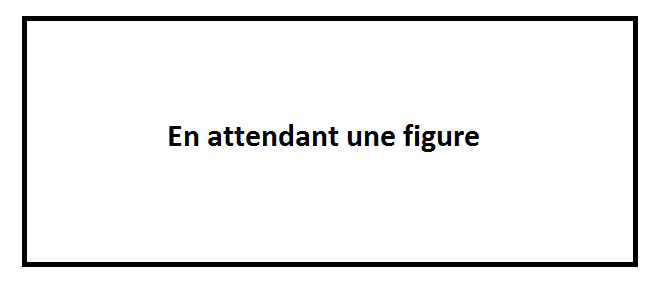
\includegraphics[height=\textheight]{En_attendant_une_figure.jpg}
	\end{titlepage}
	%\changepage{}{}{}{}{}{}{}{}{}
}{}



%%%%%%%%%%%%%%%%%%%%%%%%%%%%%
    %%  Modèle rapport         %%
    %%  Résumé                 %%
    %%  Version 2014.08.26     %%
    %%%%%%%%%%%%%%%%%%%%%%%%%%%%%


%%%%%%%%%%%%%%%%%%%%%%%%%%%%%%%%%%%%% Châpeau
\ifbool{nouvellePage}{\clearpage}{}
\section*{\nomResume}
\addcontentsline{toc}{section}{\nomResume}
\ifbool{rectoVerso}{\fancyhead[LE,RO]{\nomResume}}{\fancyhead[RE,RO]{\nomResume}}
%%%%%%%%%%%%%%%%%%%%%%%%%%%%%%%%%%%%% Texte


    Ceci est un modèle du rapport en \LaTeX.
    
    


%%%%%%%%%%%%%%%%%%%%%%%%%%%%%
    %%  Modèle rapport         %%
    %%  Table des matières     %%
    %%  Version 2014.08.26     %%
    %%%%%%%%%%%%%%%%%%%%%%%%%%%%%


\clearpage
\ifbool{rectoVerso}{\fancyhead[LE,RO]{\nomTDM}}{\fancyhead[RE,RO]{\nomTDM}}
\tableofcontents
\clearpage

    


    %%%%%%%%%%%%%%%%%%%%%%%%%%%%%
    %%  Modèle rapport         %%
    %%  Introduction           %%
    %%  Version 2014.08.26     %%
    %%%%%%%%%%%%%%%%%%%%%%%%%%%%%


%%%%%%%%%%%%%%%%%%%%%%%%%%%%%%%%%%%%% Châpeau
\ifbool{numeroIntroConclu}{
	\section{\nomIntro}
	\ifbool{rectoVerso}{\fancyhead[LE,RO]{\nomIntro}}{\fancyhead[RE,RO]{\nomIntro}}
}{
	\clearpage
	\section*{\nomIntro}
	\addcontentsline{toc}{section}{\nomIntro}
	\ifbool{rectoVerso}{\fancyhead[LE,RO]{\nomIntro}}{\fancyhead[RE,RO]{\nomIntro}}
}
%%%%%%%%%%%%%%%%%%%%%%%%%%%%%%%%%%%%% Texte



ABCDEFG\cite{lowry1951protein}


%%%%%%%%%%%%%%%%%%%%%%%%%%%%%
    %%  Modèle rapport         %%
    %%  Développement          %%
    %%  Version 2014.08.26     %%
    %%%%%%%%%%%%%%%%%%%%%%%%%%%%%


%%%%%%%%%%%%%%%%%%%%%%%%%%%%%%%%%%%%% Châpeau
\ifbool{nouvellePage}{\clearpage}{}
\chapter{AAA}
\section{A}
\ifbool{rectoVerso}{\fancyhead[LE,RO]{\leftmark}}{\fancyhead[RE,RO]{\leftmark}}
%%%%%%%%%%%%%%%%%%%%%%%%%%%%%%%%%%%%% Texte

\subsection{a}

\subsection{b}


\section{B}


\chapter{BBB}
\section{A}
\subsection{a}


\subsubsection{aaa}
\subsubsection{bbb}
\subsubsection{ccc}


\subsubsection{b}



%%%%%%%%%%%%%%%%%%%%%%%%%%%%%
    %%  Modèle rapport         %%
    %%  Conclusion             %%
    %%  Version 2014.08.26     %%
    %%%%%%%%%%%%%%%%%%%%%%%%%%%%%


%%%%%%%%%%%%%%%%%%%%%%%%%%%%%%%%%%%%% Châpeau
\ifbool{numeroIntroConclu}{
	\section{\nomConclu}
	\ifbool{rectoVerso}{\fancyhead[LE,RO]{\nomConclu}}{\fancyhead[RE,RO]{\nomConclu}}
}{
	\clearpage
	\section*{\nomConclu}
	\addcontentsline{toc}{section}{\nomConclu}
	\ifbool{rectoVerso}{\fancyhead[LE,RO]{\nomConclu}}{\fancyhead[RE,RO]{\nomConclu}}
}
%%%%%%%%%%%%%%%%%%%%%%%%%%%%%%%%%%%%% Texte

AAAAAAAAAAAAAAAAAAAAAAAAAAAAAAAAAAAAA

BBBBBBBBBBBBBBBBBBBBBBBBBBBBBBBBBBBBB

    
    


%%%%%%%%%%%%%%%%%%%%%%%%%%%%%
    %%  Modèle rapport         %%
    %%  Remerciement           %%
    %%  Version 2014.08.26     %%
    %%%%%%%%%%%%%%%%%%%%%%%%%%%%%


%%%%%%%%%%%%%%%%%%%%%%%%%%%%%%%%%%%%% Châpeau
\ifbool{numeroRemerci}{
	\section{\nomRemerci}
	\ifbool{rectoVerso}{\fancyhead[LE,RO]{\nomRemerci}}{\fancyhead[RE,RO]{\nomRemerci}}
}{
	\clearpage
	\section*{\nomRemerci}
	\addcontentsline{toc}{section}{\nomRemerci}
	\ifbool{rectoVerso}{\fancyhead[LE,RO]{\nomRemerci}}{\fancyhead[RE,RO]{\nomRemerci}}
}
%%%%%%%%%%%%%%%%%%%%%%%%%%%%%%%%%%%%% Texte


    Le stage que j'ai effectué n'aurait pu être mené à bien sans l'aide précieuse que plusieurs interlocuteurs ont apportée au cours de mon travail.

    J'exprime d'abord mes remerciements à mon ordinateur Caroline pour son travail assidu et sa performance impeccable. Elle reste toujours à mon côté malgré un accident de chute libre à partir de 1 mètre du sol. Pour son sacrifice, ses peines et son dévouement, je lui suis très reconnaissant.

    Je voudrais remercier arXiv.org pour avoir assuré la partie théorique de mon travail. Il a eu la gentillesse d'accroître ma liste de la bibliographie à étudier de façon exponentielle. Pour son zèle en éclaircissement du sujet, je souhaite manifester ma pleine gratitude.

    Je remercie sincèrement Facebook pour son divertissement personnalisé. Son interface bleue m'a secouru plusieurs fois de la fenêtre noire de la terminale où je me noyais. Ses efforts en distraction tout au long du stage m'ont été indispensables.

    Je remercie davantage la collection Folio pour ses {\oe}uvres riches d'intérêts, sans quoi je serais mort d'ennui pendant les grèves mensuelles et les accidents hebdomadaires de l'ensemble du réseau ferré parisien. Pour son esprit sacré de combattre le transport en commun à Paris, je lui exprime ma considération distinguée.

    Je voudrais également remercier le restaurant CROUS Paris - Halles aux Farines pour sa gastronomie de bon marché. Contrairement au plat à 5 raviolis d'une certaine cantine palaisienne, il a eu la volonté de montrer sa qualité notamment en rapport quantité-prix. Sa générosité inouïe m'a été très précieuse.

    Je tiens particulièrement à remercier les chercheuses italiennes du bureau à deux pas, pour leurs défilés de mode et leurs conversations charmantes bien que incompréhensibles.

    Merci enfin à tous ceux qui ont croisé le chemin de mon stage, s'y sont intéressés et ont contribué à le faire avancer à divers titres, par leur curiosité et ou leur sympathie.



%%%%%%%%%%%%%%%%%%%%%%%%%%%%%
    %%  Modèle rapport         %%
    %%  Annexe                 %%
    %%  Version 2015.06.28     %%
    %%%%%%%%%%%%%%%%%%%%%%%%%%%%%


%%%%%%%%%%%%%%%%%%%%%%%%%%%%%%%%%%%%% Châpeau
\clearpage
\appendixpage
\addappheadtotoc
\ifbool{rectoVerso}{\fancyhead[LE,RO]{\nomAnnexe}}{\fancyhead[RE,RO]{\nomAnnexe}}
%%%%%%%%%%%%%%%%%%%%%%%%%%%%%%%%%%%%% Configurations post-châpeau
\titleformat{\subsection}[hang]{\large\bf}{\color{couleurSubsection}\Alph{subsection}}{5mm}{\color{couleurSubsection}} %% Pour le titre
\renewcommand{\thesubsection}{\textcolor{couleurSubsection}{\Alph{subsection}}} %% Pour la table des matières
\ifbool{compteurFigTabAvecSec}{ %% Pour les compteurs de figures et de tableaux
	\numberwithin{figure}{subsection} %% Ajouter le numéro de la subsection pour les figures
	%\renewcommand{\thefigure}{\Alph{subsection}.\arabic{figure}} %% Changement du style si nécessaire
	\numberwithin{table}{subsection} %% Ajouter le numéro de la subsection pour les tableaux
	%\renewcommand{\thetable}{\Alph{subsection}.\arabic{table}} %% Changement du style si nécessaire
}{}
%%%%%%%%%%%%%%%%%%%%%%%%%%%%%%%%%%%%% Texte


%% A %%
\subsection{Calcul bourrin}

    \begin{table}[!htb]
        \centering \begin{tabular}{|ccc|}
            \hline
            A & B & C \\
            \hline
            data & data & data \\
            data & data & data \\
            data & data & data \\
            \hline
        \end{tabular}
        \caption{Légende}
        \label{etiquette3}
    \end{table}

    Voici des exemples:
    \begin{itemize}
        \item ex1;
        \item ex2.
    \end{itemize}

    \vspace*{1ex}
    Paragraphe.
    
    


%%%%%%%%%%%%%%%%%%%%%%%%%%%%%
    %%  Modèle rapport         %%
    %%  Bibliographie          %%
    %%  Version 2016.04.10     %%
    %%%%%%%%%%%%%%%%%%%%%%%%%%%%%


%%%%%%%%%%%%%%%%%%%%%%%%%%%%%%%%%%%%% Châpeau
\clearpage
\selectlanguage{english}
\renewcommand{\refname}{\nomBiblio} %% Doit être après \selectlanguage{English}
\addcontentsline{toc}{section}{\nomBiblio}
\ifbool{rectoVerso}{\fancyhead[LE,RO]{\nomBiblio}}{\fancyhead[RE,RO]{\nomBiblio}}
%%%%%%%%%%%%%%%%%%%%%%%%%%%%%%%%%%%%% Texte


\ifnumequal{\entreeBiblio}{1}{ %% Bibliographie avec .bib
	\bibliography{biblio}
}{}

\ifnumequal{\entreeBiblio}{2}{ %% Bibliographie indépendante
	\begin{thebibliography}{99}

    \bibitem[NomDeLAuteur (1999)]{Revue}
        NomDeLAuteur, Prenom.
        \emph{NomDeLArticle}.
        NomDeLaRuvue, Vol.XX, No.YY, p.ZZ.
        NomDeLEdition.
        Année.

    \bibitem{Livre}
        NomDeLAuteur, Prenom.
        \emph{NomDuLivre}.
        NomDeLEdition.
        Année.

    \bibitem{Conference}
        NomDeLAuteur, Prenom.
        \emph{TitreDuSujet}.
        NomDeLaConference.
        Lieu.
        Année.

	\end{thebibliography}
}{}


\iffalse\fi


\end{document}

